\newcommand{\source}[1]{\caption*{Source: {#1}} }

\section{Verwandte Arbeiten}\raggedbottom

\subsection{Semantische Segmentierung im medizinischen Bereich}

\subsubsection{Semantische Segmentierung}

Die semantische Segmentierung erfolgt in drei Schritten:

Klassifizierung: Klassifizierung eines bestimmten Objekts im Bild.
Lokalisieren: Auffinden des Objekts und Zeichnen eines Begrenzungsrahmens um das Objekt.

Segmentierung: Gruppierung der Pixel in einem lokalisierten Bild durch Erstellung einer Segmentierungsmaske.

Im Wesentlichen kann man die Aufgabe der semantischen Segmentierung als Klassifizierung einer bestimmten Bildklasse und deren Abgrenzung von den übrigen Bildklassen durch Überlagerung mit einer Segmentierungsmaske bezeichnen.

Allgemein kann man es sich auch als Klassifizierung von Bildern auf Pixelebene vorstellen.

\subsubsection{Medizinischer Bereich}

Die medizinische Bildgebung umfasst viele Kategorien, von 2- bzw. 3 dimensionalen MRT Scans des Herzens, Gehirns und des Magen-Darm Trakts, 2 dimensionalen Röntgen Bildern sowie Ausschnitte aus der Videoendoskopie.

Bereits in den 90er Jahren wurde sich mit mit Segmentierungsarchitekturen auseinandergesetzt und baselines geschaffen. Zu dieser Zeit lieferten Methoden im Bereich \glqq Pattern recogniction\grqq die besten Ergebnisse. Die Autoren legten viel Wert auf preprocessing der Daten und werteten die zu jener Zeit besten Modelle aus. Es handelte sich um einen Feature basierten Ansatz, es wurden Algorithmen wie
\href{https://en.wikipedia.org/wiki/K-nearest_neighbors_algorithm}{kNN},
\href{https://en.wikipedia.org/wiki/Maximum_likelihood_estimation}{Maximum Likelihood} und
\href{https://en.wikipedia.org/wiki/Eigenvalues_and_eigenvectors}{Characteristic vector} getestet.

Trotz aller Bemühungen wiesen die Modelle nur eine Accuracy von 3\% bis 34\% auf. \citep{Clarke:Mri1995}

Jedoch waren die Autoren davon überzeugt, dass segmentierung eine wichtige Rolle im Beriech der Verarbeitung von MRT Daten darstellen wird und mit wachsender Akzeptanz auf klinischer Seite sowie dem technischen Fortschritt der Hochleistungsrechner es in Zukunft möglich sein wird, akkurate Segmentierungen von MRT Scans im Livebetrieb vorzunehmen.

\newpage

\subsection{Deep Learning-Techniken für die Segmentierung medizinischer Bilder:
Errungenschaften und Herausforderungen}

Dank der immensen Verbesserung der Rechenleistung der Hardwarecomponenten wurde das Thema Deep Learning immer interessanter und gehört heutzutage zur standard Herangehensweise. Architekturen wie das U-Net Modell \citep{U-Net} haben sich hierbei besonders bewiesen und wurden mit den Jahren nach der Veröffentlichung in 2015 stetig erweitert, so dass es für viele verschiedene (medizinische) Bereiche Architekturen vorliegen, die auf die jeweiligen Problemstellungen angepasst wurden, jedoch trotzdem Anwendung auf ähnlichen Gebieten finden können \citep{Hesamian}

\subsection{Intelligentes Zuschneiden des Inputs}

Dimitrios G. Zaridis et al. \citep{SmartCrop} haben sich ebenfalls mit verschiedenen State of the Art U-Net Architekturen auseinandergesetzt und eine Baseline geschaffen. Trotz der beachtlichen Leistung, die die Modelle liefern, sind sie der Meinung dass noch Verbesserungspotential vorhanden ist.

Sie fanden heraus, dass das Vorhandensein eines Klassenungleichgewichts, wo der Anteil der Hintergrundpixel dem Anteil des zu segmentierenden Organs überwiegt zu Problemem führen kann. Mithilfe eines Deep Learning Modells haben die Autoren es geschafft, dieses Klassenungleichgewicht zu reduzieren, in dem das Neuronale Netzwerk die gesuchten Organe lokalisiert, das Originalbild zuschneidet und am Ende das Verhältnis von Vorder- und Hintergrundpixeln normalisiert. Dies führte bei allen gängigen Deep Learning Netzwerken zu erheblichen Verbesserung im Bezug des Dice-Scores. U-Net+ und ResU-Net++ wiesen mithilfe dieser Technologie Verbesserungen von bis zu 8\% auf.

\section{Grundlagen}\raggedbottom

\subsection{Magen-Darmtrakt}

Um die Daten zu verstehen und Erkentnisse aus den Ergebnissen zu gewinnen, ist es wichtig ein Grundverständnis für den Bereich des Körpers zu haben, den unsere Daten beschreiben. Wir interessieren uns in unserem Fall für den Dick- bzw. Dünndarm sowie den Magen. Hierbei liegt die Herausforderung, dass je nach Ernährungsverhalten, Schlafposition, anderen Krankheiten und Verdauung die Position der Organe stark (bzw. stärker als andere) variieren kann. Mithilfe der Grafik kann man sich ein Bild vom groben Aufbau machen. \autoref{magen-darm-trakt}

\begin{figure}[htb]
	\begin{center}
		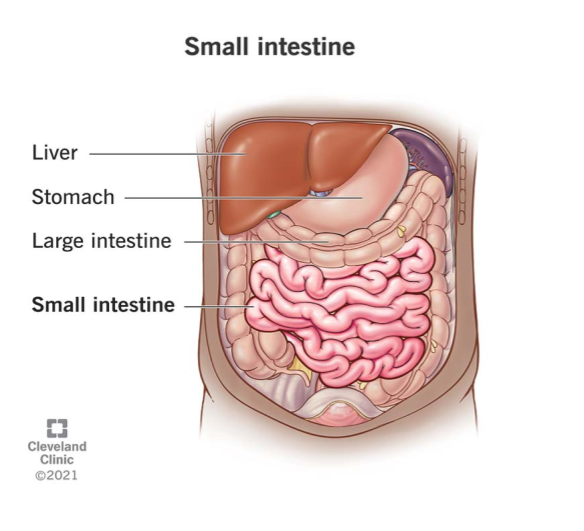
\includegraphics[width=450pt]{bilder/intestines}
		\caption{Magen-Darm Trakt}\label{magen-darm-trakt}
	\end{center}
\end{figure}

\begin{figure}[htb]
	\begin{center}
		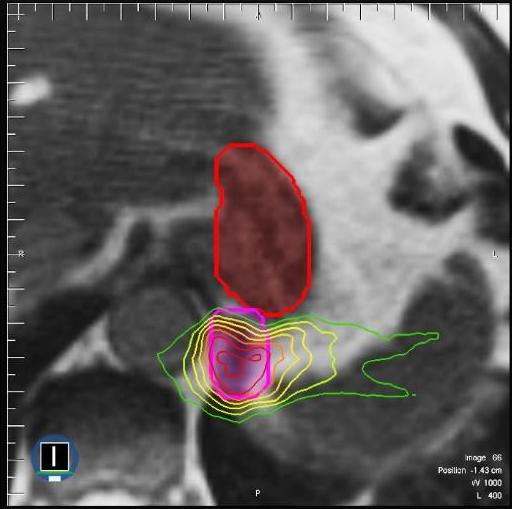
\includegraphics[width=450pt]{bilder/magen-mrt}
		\caption{Beispiel MRT des Magen-Darm Traks. Zu sehen ist der Magen (rot) und der Tumor (pink) sowie die verabreichte Strahlendosis. Die Strahlenintensivität werden durch den Regenbogen der Umrisse dargestellt, wobei höhere Dosen rot und niedrigere Dosen grün dargestellt werden.}\label{magen-mrt}
	\end{center}
\end{figure}

\subsection{U-Net}
% CNN, Convolution, Maxpooling oder ReLu erklären?

U-Net wurde im Jahr 2015 von Olag Ronneberger et al. \citep{U-Net} vorgestellt als Segmentierungsarchitektur für den biomedizinischem Bereich und bildet die Baseline dieser Arbeit. Neu in der Herangehensweise ist der Encoder-Decoder Part, die dem Netzwerk ermöglicht räumliche Merkmale anzutrainieren.
Klassisch handelt es sich um ein
\href{https://en.wikipedia.org/wiki/Convolutional_neural_network}{Convolutional Neural Network}, bestehend es aus 5 bis 6 \glqq downsampling\grqq Schichten (auch Encoder genannt)  und der gleichen Menge an \glqq upsampling\grqq Schichten (auch Decoder genannt).

Eine \glqq downsample\grqq  Operation besteht zum einen aus einer
\glqq \href{https://en.wikipedia.org/wiki/Convolution}{Convolution Operation}\grqq
sowie einer
\glqq \href{https://computersciencewiki.org/index.php/Max-pooling_/_Pooling}{Max Pooling}\grqq
an deren Ende jeweils eine
 \glqq \href{https://deepai.org/machine-learning-glossary-and-terms/relu}{ReLu}\grqq
 Aktivierungsfunktion zum Einsatz kommt. In diesem Schritt lernt das Modell Eigenschaften auf Pixelebene, wie zum Beispiel Formen, Ecken, Kanten. Hierbei halbieren sich die Eingabedimensionen und die Tiefe des Bildes wird erhöht. Veranschaulicht kann man sagen, dass das Modell das \glqq Was\grqq lernt, was im Bild zu sehen ist. \citep{Con97} Zur Semantischen Segmentierung fehlt dann nur noch das  \glqq Wo\grqq, hierbei wird das Zusammenspiel von En- und Decoder deutlich.

Im Decoder wird das Bild wieder auf seine ursprüngliche Größe mittels 
\glqq \href{https://en.wikipedia.org/wiki/Deconvolution}{Transpose Convolution operations}\grqq  
gebracht. Hier ersetzt die transponier Operation die Maxpooling Operation (vergleich Grafik). Dieser Part erlaubt dem Modell das lokalisieren der zuvor gelernten Eigenschaften. Output ist eine Maske, bestehend aus Nullen und Einsen, die der Eingabegröße gleicht und bestenfalls den Wert Eins an der Stelle des gesuchten Organs enthält.

\begin{figure}[htb]
	\begin{center}
		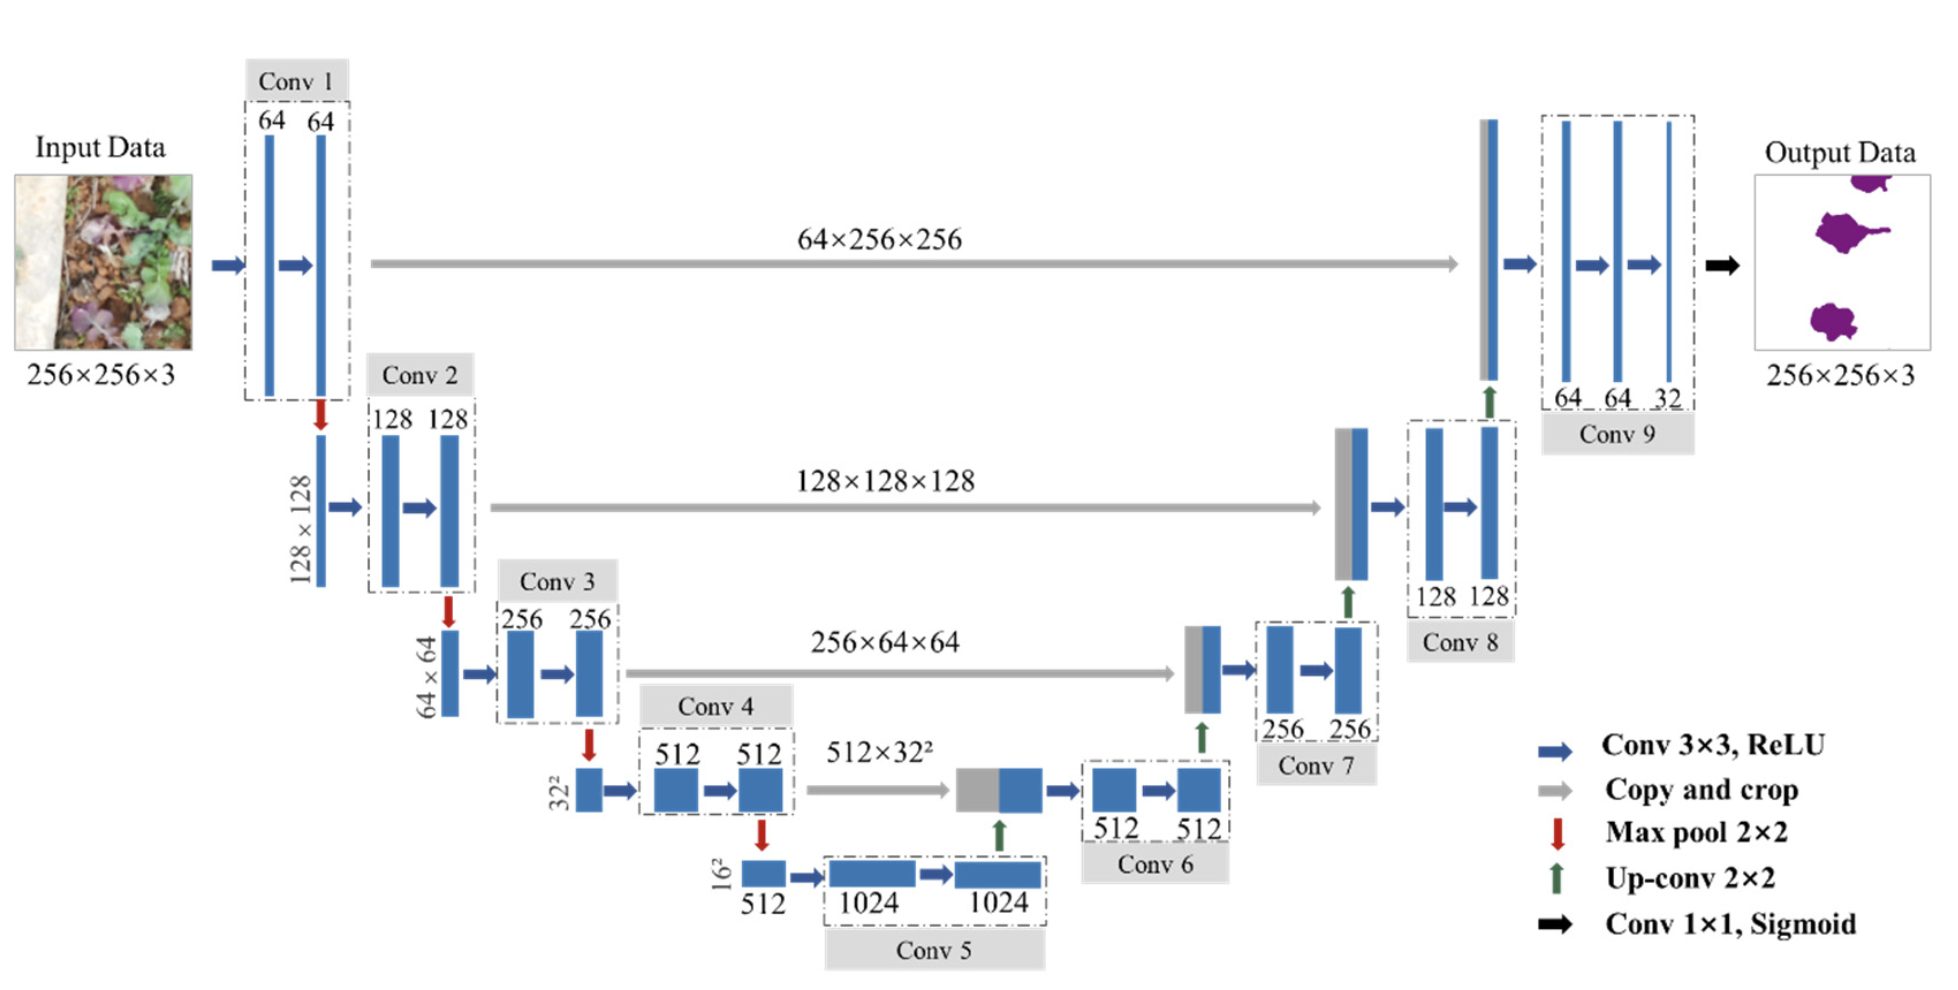
\includegraphics[width=300pt, angle=270]{bilder/u-net-architecture}
		\caption{U-Net Architektur}\label{Fig:unet-diagram}
	\end{center}
\end{figure}

\subsection{Encoder 1}
Eventuell

\subsection{Encoder 2}
Eventuell


\section{Methodik}\raggedbottom

\subsection{Datenanalyse}
Der Datensatz besteht aus 115 488 Zeilen und enthält drei features: ID, Klasse und einem Run-lenght codierten String, der die Maske enthält. \autoref{tabelle_daten}. Jeder ID sind drei Zeilen gewidmet, jeweils für die drei Klassen. Zu jeder ID existiert ein Graustufen Bild, welche sich im train Ordner befinden:

input\textbackslash uw-madison-gi-tract-image-segmentation\textbackslash train\textbackslash case101\textbackslash \\case101\textunderscore
day20\textbackslash scans\textbackslash slice\textunderscore 0001\textunderscore 266\textunderscore 266\textunderscore 1.50\textunderscore 1.50.png

Ein Beispiel der Ordnerhierarchie kann man hier sehen \autoref{Fig:train-data}

\begin{figure}[htb]
	\begin{center}
		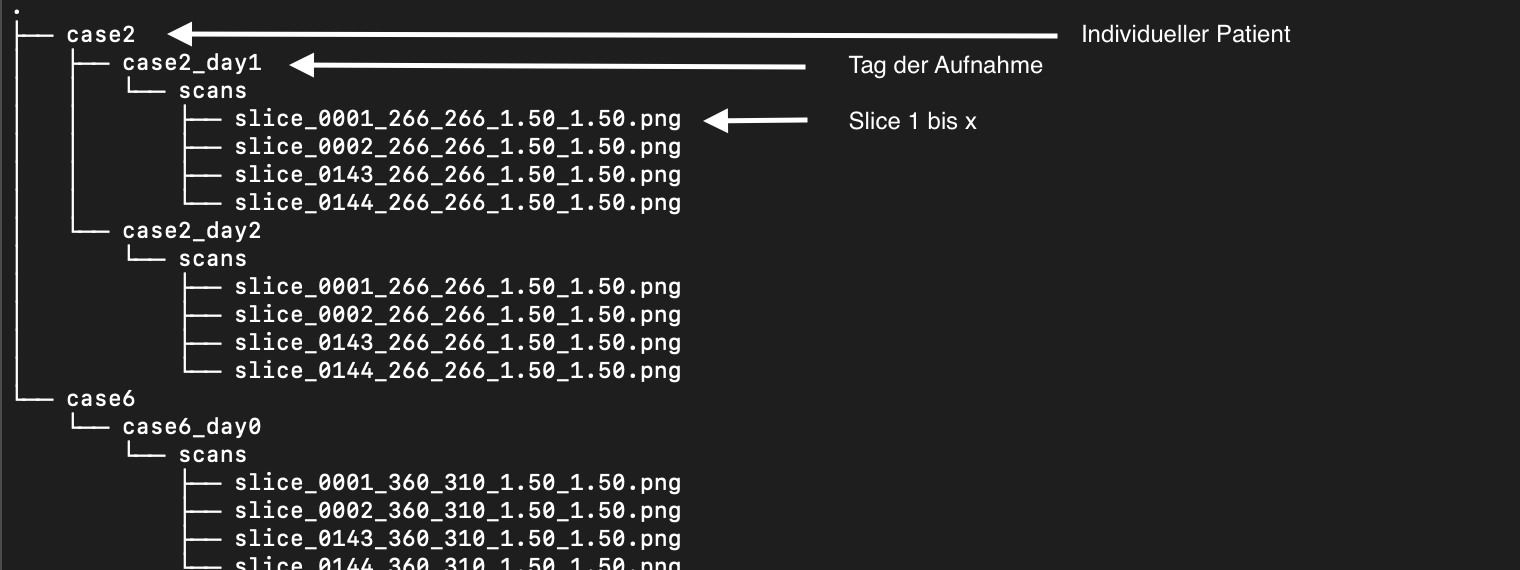
\includegraphics[width=450pt]{bilder/data_tree}
		\caption{Trainingsdaten Hierachie}\label{Fig:train-data}
	\end{center}
\end{figure}

Jedes slice enthält vier Zahlen (z.B. 266\textunderscore 266\textunderscore 1.50\textunderscore 1.50.png), die ersten beiden stehen für die Auflösung des Bildes und die letzten beiden für den physischen Abstand der Pixel. Der Großteil der Aufnahmen stammt von Tag null oder tag eins \autoref{Fig:slice_per_day} und die durchschnittliche Anzahl an Bildern pro Fall beträgt X.

Beim betrachten der Verteilung der Segmentierungen fällt auf, dass das Vorkommen für jede Klasse stark variiert. \autoref{Fig:klassenverteilung}.

\begin{figure}[htb]
	\begin{center}
		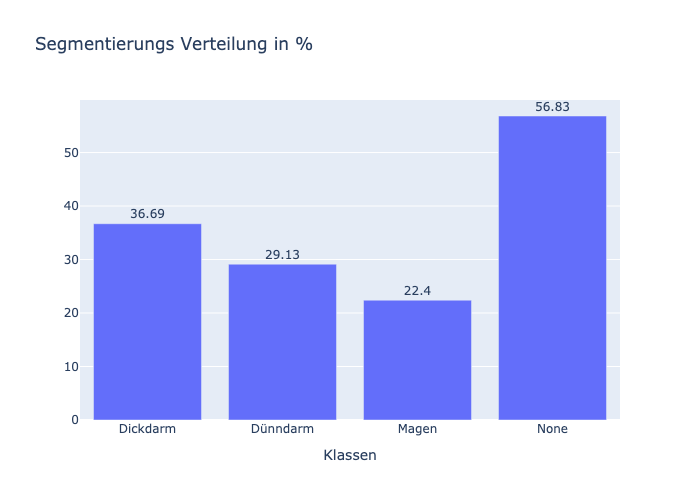
\includegraphics[width=220pt , angle=270]{bilder/segmentation_distribution}
		\caption{Verteilung der Klassen im Testset}\label{Fig:klassenverteilung}
	\end{center}
\end{figure}

\begin{table}[]
	\begin{center}
	        \small
	        \setlength\tabcolsep{2pt}
		\begin{tabular}{|c|c|c|c|c|c|c|c|c|}
			\hline
			Index  & ID & Class & Segmentation \\
			\hline \hline
			1     & case134\textunderscore day0\textunderscore slice\textunderscore 0085 	& large\textunderscore bowel 	&  NaN  \\
			2     & case134\textunderscore day0\textunderscore slice\textunderscore 0085 	& small\textunderscore bowel 	&  41591 5 41599 7 41949 27 ...  \\
			3     & case134\textunderscore day0\textunderscore slice\textunderscore 0085 	& stomach 	&  NaN \\
			4     & case123\textunderscore day0\textunderscore slice\textunderscore 0001 	& large\textunderscore bowel 	&  35223 6 74352 7 32312 12 ...   \\
			5     & case123\textunderscore day0\textunderscore slice\textunderscore 0001 	& small\textunderscore bowel 	&  63432 5 12354 7 41949 12 ...  \\
			6     & case123\textunderscore day0\textunderscore slice\textunderscore 0001 	& stomach 	&  NaN \\
			\hline
		\end{tabular}
		\caption{Beispieldaten für zwe slices}\label{tabelle_daten}
	\end{center}
\end{table}

\begin{figure}[!htb]
   \begin{minipage}{0.48\textwidth}
     \centering
     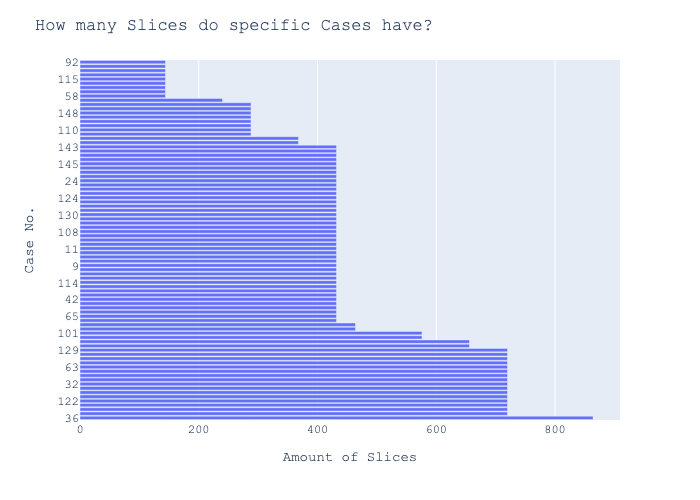
\includegraphics[width=1.2\linewidth]{bilder/slice_per_case}
     \caption{Anzahl Bilder pro Fall}\label{Fig:slice_per_case}
   \end{minipage}\hfill
   \begin{minipage}{0.48\textwidth}
     \centering
     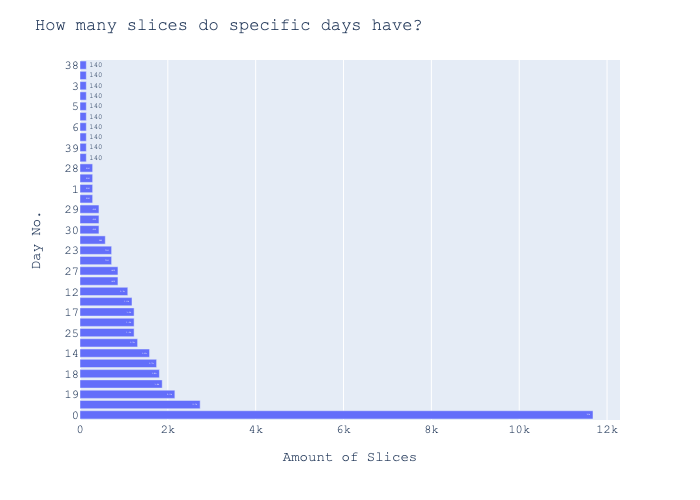
\includegraphics[width=1.2\linewidth]{bilder/slices_per_day}
     \caption{Anzahl Bilder pro Tag}\label{Fig:slice_per_day}
   \end{minipage}
\end{figure}

\subsection{Metadatenextraktion}

Anhand der ID eines jedes Slices war es möglich verschiedene Metadaten dem originalem Dataframe zu entziehen, zudem wurde die gesamtlänge gedrittelt, dadurch dass die Klassen einer ID  zugewiesen worden sind. \autoref{tabelle_meta_daten}


% & rs & re & cs & ce & count & path00 & path01 & path02 & image\textunderscore paths

\begin{table}[]
 \begin{center}
  \scalebox{0.7}{
   \begin{tabular}{|l|l|l|l|l|l|l|l|l|l|l|l|l|l|}
     \hline
     Idx  & ID &  large\textunderscore bowel & small\textunderscore bowel & stomach & case & day & slice & path & width & height & pixel\textunderscore x & pixel\textunderscore y \\
     \hline \hline
     1     & case134\textunderscore day0\textunderscore slice\textunderscore 0085 	& NaN & 41591 5  ...    & NaN & 134 & 0 & 85 & input\textbackslash  & 266 & 266 & 1.5 & 1.5  \\
     2     & case134\textunderscore day0\textunderscore slice\textunderscore 0086 	& 41591 27 ... & NaN    & NaN & 134 & 0 & 86 & input\textbackslash  & 266 & 266 & 1.5 & 1.5  \\
     3     & case134\textunderscore day0\textunderscore slice\textunderscore 0086 	& NaN & NaN   & NaN & 134 & 0 & 87 & input\textbackslash  & 266 & 266 & 1.5 & 1.5  \\
     \hline
   \end{tabular}
   }
   \caption{Metadaten für drei slices}\label{tabelle_meta_daten}
 \end{center}
\end{table}

\pagebreak

\subsection{Algorithmik}

Dieses Projekt wurde gänzlich in Python mithilfe der TensorFlow API sowie dem
 \href{https://deepai.org/machine-learning-glossary-and-terms/relu}{Segmentation Models} \citep{Yakubovskiy:2019}
 Package aufgezogen, welches verschiedene Architekturen und an- oder nicht antrainierte Encoder zur verfügung stellt. Trainiert wurde mit dem
\href{https://optimization.cbe.cornell.edu/index.php?title=Adam}{Adam Optimizer},
 und einer initialen Learning Rate von von 5e-4, die sich um den Faktor e-1 verringert, wenn sich der Validation-loss nach fünf Epochen unverändert schlecht bleibt. Die Loss function ist eine Mischung aus 
\href{https://www.analyticsvidhya.com/blog/2021/03/binary-cross-entropy-log-loss-for-binary-classification/}{Binary Crossentropy} und zu 50\%
Dice Loss. Diese Kombination eignet sich laut Jadon  \citep{Jadon_2020} besonders gut, um Segmentierungsarchitekturen anzulernen. Ansonsten wurde mit einer Batchsize von 16 und 32 trainiert.
Die Daten wurden mithilfe von der 
\href{https://scikit-learn.org/stable/modules/generated/sklearn.model_selection.StratifiedGroupKFold.html}{StratifiedGroupKFold} Methode von Sklearn in 5 Folds aufgeteilt und nach Case gruppiert. Somit 
wurde das Verhältnis der Klassendistribution in jedem Fold beibehalten. 

\subsection{2.5 dimensionale Daten}
?

\subsection{Intelligentes Zuschneiden}
?

\subsection{Nachbearbeitung }
?

\subsection{Experimente}
Experimente.

\section{Evaluation}\raggedbottom

\section{Fazit}\raggedbottom

\subsection{Ausblick}
Ideen, die es nicht in die Arbeit geschafft haben oder nicht schafffen konnten.


\ifthenelse{\boolean{\biber}}{ % Beispiel um mit Biber zu zitieren (\citet und \citep)
	\citet{Con97} hat ein Buch geschrieben. Es gibt auch andere Arbeiten \citep{PeHe97} die referenziert sind. In Abbildung \ref{fig_Gallien} ist ein Sachverhalt dargestellt.


	1 Autor: \citet{Con97} \hspace*{1cm} \citep{Con97}\\
	2 Autoren: \citet{IWNLP} \hspace*{1cm} \citep{IWNLP}\\
	3 Autoren: \citet{liebeck-esau-conrad:2016:ArgMining2016} \hspace*{1cm} \citep{liebeck-esau-conrad:2016:ArgMining2016}

	Online resource: \citet{ILSVRC2016}
}{ %  Beispiel um klassisch zu zitieren (\cite)
	\cite{Con97} hat ein Buch geschrieben. Es gibt auch andere Arbeiten \cite{PeHe97} die referenziert sind. In Abbildung \ref{fig_Gallien} ist ein Sachverhalt dargestellt.


	1 Autor: \cite{Con97} \hspace*{1cm} \cite{Con97}\\
	2 Autoren: \cite{IWNLP} \hspace*{1cm} \cite{IWNLP}\\
	3 Autoren: \cite{liebeck-esau-conrad:2016:ArgMining2016} \hspace*{1cm} \cite{liebeck-esau-conrad:2016:ArgMining2016}

	Online resource: \cite{ILSVRC2016}
}

\ifthenelse{\equal{\sprache}{deutsch}}{
	\textbf{quotes}:\\
	Ein Beispiel für deutsche Anführungszeichen \glqq quote\grqq.
}{}

\pagebreak
